%% The first command in your LaTeX source must be the \documentclass command.
%%
%% Options:
%% two-column: Two-column layout.
%% hf: enable header and footer.
\documentclass[
% twocolumn,
% hf,
]{ceurart}
\usepackage{amsmath,amssymb,longtable,hhline}
\usepackage{doi}
\def\doitext{DOI:}

%%
%% One can fix some overfills
\sloppy

%%
%% Minted listings support
%% Need pygment <http://pygments.org/> <http://pypi.python.org/pypi/Pygments>
% \usepackage{listings}
\usepackage{minted}
\setminted{fontsize=\footnotesize,mathescape}
\usepackage{hyperref}
\usepackage{multicol}

\hypersetup{
    bookmarks=true,         % show bookmarks bar?
    unicode=true,           % non-Latin characters in Acrobat’s bookmarks
    pdftoolbar=false,        % show Acrobat’s toolbar?
    pdfmenubar=false,        % show Acrobat’s menu?
    pdffitwindow=false,     % window fit to page when opened
    pdfstartview={FitH},    % fits the width of the page to the window
    pdftitle={},    % title
    pdfauthor={Evgeny Cherkashin},     % author
    pdfsubject={Technologies of Semantic WEB as an environment of application development and integration},   % subject of the document
    pdfnewwindow=true,      % links in new PDF window
    colorlinks=true,       % false: boxed links; true: colored links
    linkcolor=red,          % color of internal links (change box color with linkbordercolor)
    citecolor=green,        % color of links to bibliography
    filecolor=magenta,      % color of file links
    urlcolor=blue           % color of external links
  }

\usepackage{pifont}
\usepackage{xcolor}
\graphicspath{{pics/}}

\newcommand{\GB}[1]{\colorbox{green}{#1}}
\newcommand{\BB}[1]{\colorbox{blue}{#1}}
\newcommand{\RB}[1]{\colorbox{red}{#1}}


%% auto break lines
% \lstset{breaklines=true}

\newcommand{\ns}[1]{\textbf{\texttt{#1}}}

%%
%% end of the preamble, start of the body of the document source.
\begin{document}

%%
%% Rights management information.
%% CC-BY is default license.
\copyrightyear{2021}
\copyrightclause{Copyright for this paper by its authors.
  Use permitted under Creative Commons License Attribution 4.0
  International (CC BY 4.0).}

%%
%% This command is for the conference information
\conference{2nd International Workshop on Advanced Information and Computation Technologies and Systems, December XX--XX, 2021, Irkutsk, Russia}

%%
%% The "title" command
\title{Technologies of Semantic WEB as an environment of application development and integration}
%%
%% The "author" command and its associated commands are used to define
%% the authors and their affiliations.
\author[1,2]{Evgeny A. Cherkashin}[%
orcid=0000-0003-2428-2471,
email=eugeneai@icc.ru,
url=https://github.org/eugeneai,
]
\address[1]{Matrosov Institute for System Dynamics and Control Theory of Siberian Branch of Russian Academy of Sciences, 134 Lermontov St, Irkutsk, 664033, Russian Federation}

\address[2]{Institute for Mathematics and Information Technologies, Irkutsk State University, 20~Gagarina Bulv, Irkutsk, 664003, Russian Federation}

%%
%% The abstract is a summary of the work to be presented in the
%% article.
\begin{abstract}
  Semantic Web technologies and their standards are becoming productive assets for software development and integration on various design and implementation levels.  These include OSI level 6 data representation, database and file storage formats, the source data for text indexes, document authoring, hypertext markup engines, a representation for abstract software models, \emph{etc.}  They are also smoothly combined with the development and data analysis tools, giving rise to a new common-ground environment for integrating distributed applications on a semantic level.

  This paper presents a view on the Semantic Web technologies as data representation for software development tools with model analysis, transformation, and retrospection capabilities.  Three examples show the technologies usage, exposing our experience.
\end{abstract}

%%
%% Keywords. The author(s) should pick words that accurately describe
%% the work being presented. Separate the keywords with commas.
\begin{keywords}
  knowledge graph \sep
  semantic web \sep
  model transformation \sep
  model-driven architecture \sep
  object-oriented logical programming \sep
  web application \sep
  geographical information system
\end{keywords}


%%
%% This command processes the author and affiliation and title
%% information and builds the first part of the formatted document.
\maketitle

\section{Introduction}

Since 2001 \cite{tbl}, the Semantic Web (SW) technologies have become actively used in describing software domains, representing semantic relations between objects.  First-order knowledge theories are constructed for some domains based on the SW description, but in the practical aspect of the SW utilization, the solving data representation problems and software integration aspects prevail.  Some tools for automation of conceptual model design and model conversion were proposed \cite{hogan}.  The R\&D at present are carried on in developing applications, improving and standardizing vocabularies (conceptual domain models), devising tools for solving particular problems.

Unification of routine tasks resulted in standard development techniques for storing and processing data aggregated around the term ``knowledge graph'' (KG).  These include data representation formats, vocabulary standards, query languages, tools for accessing and managing data in a KG.  Software development techniques are mediated with properties of the new-created resources and their APIs\footnote{Abbreviation of Application Programming Interface}.  Many internet resources provide standard ways of formalized domain data access using query endpoints, and these endpoints allow one to organize federated KG data access.

In Russia, domain model designers generally prefer to develop local vocabularies instead of spending time for the routine work of Internet surfing for existing conceptual models and their enrichment.  It is due to underdevelopment of the metadata resources (metavocabularies) due to lack of a domain classification system as compared, \emph{e.g.} to Universal Decimal Classification (UDC) used in the bibliography.  Vocabularies also can have common parts, describing the same or similar entities with different terms and relations, \emph{e.g.} semantically more adapted to a specific problem-solving.

Unitizing standardized vocabularies as conceptual domain models (ontologies) in our projects allows us to compare other research groups' points of view to a problem with a formalized context and figure out underestimated and not fully formularized aspects of a domain under investigation or automation.  The vocabularies are similar to information sources as scientific papers but have a concrete formal presentation of the information objects, allowing one to get rid of particular uncertainties.  Another advantage of standardization is constructing a common ground of research, development, data formalization, and interchange formats and semantics.  It includes an aggregation of pattern recognition results applications of machine learning with their following use as facts in knowledge-based systems.

This paper aims to present a contemporary experience of SW and KG utilization in the development of applications in a context of performance improvement of R\&D.  Three examples were reviewed, showing good points of the technologies' application.


\section{Semantic Web tools}
\label{sec:sw-tools}

Briefly, SW technologies from a developer point of view include the following assets:
\begin{enumerate}
\item Global identification of the entities via URI\footnote{Abbreviation of Universal Resource Identifiers}, IRI\footnote{Abbreviation of International Resource Identifier}, URL\footnote{Abbreviation of Universal Resource Locator}, which are essentially the same notions but reflecting different representation properties of an identified resource;
\item Conceptual set-theoretic and category-theoretic data representation notation as relations between resources and literals represented with triples of a form \texttt{<subject, predicate, object>};
\item Triples used in a description of a domain form a corresponding semantic graph, conditionally subdivided into terminological subgraph (T-Box) and instance subgraph (A-Box);
\item Graph presentation formats and techniques are implemented in files, databases, markups of documents, a data flow between applicants; \label{kg1}
\item There are public semantic databases comprising the generic domain objects descriptions, which are mostly A-Boxes (databases), for example, \texttt{DBPedia.org}, a formalized version of \texttt{Wikipedia.org}. % wikidata
\item For graphs being databases, query services are implemented to allow users to obtain its data by portions, as well as implement modifications;
\item API and libraries for processing files and documents with semantic data acquisition (\emph{e.g.} by extraction of the markup).
\item Software for graph data processing to improve its structure or induct general relation patterns;
\item Validation and verification services allow one to explore consistency and completeness of the conceptual domain models and their implementations in software. \label{kg2}
\end{enumerate}
The assets  \ref{kg1}--\ref{kg2} form knowledge graph technological aspect of the SW that gained a particular interest within R\&D in the last decade.

Each entity described in SW has its unique global IRI, its virtual or real internet address.  Document entities' resource IRIs are formed accounting the document structure, \emph{e.g.} a hierarchy of contexts.  Using IRIs in applications solves the fundamental problem of cross-domain and cross-application object identification and forms a basis for a standardized data processing environment.  Entities of various abstract levels can be designated an IRI, including vocabulary definitions (\emph{namespaces}), data types, data containers (files, databases).

Triples are a combination of two or three IRIs (\texttt{<subjectIRI, predicateIRI, object>}).  Subject and predicate are always IRIs, whereas objects are either IRI (a reference to a resource) or a literal.  Literals are values of basic types (\emph{e.g.}, number, string, date, time) usually accompanied with metadata (type designator or a language tag).  Types are defined in a vocabulary \texttt{<\url{http://www.w3.org/2001/XMLSchema}\#>}, having well-known namespace abbreviation \ns{xs}\footnote{Hereafter, all well-known namespace names will be written with a bold monospace font.}.  A language tag defines string values attribute, affiliating them to a cultural context.  It is recognized with KG tools and utilized at presentation layers of the software.

Namespaces are convenient instruments in the triple definition.  For example \verb|integer| literal \verb|42^^<http://www.w3.org/2001/XMLSchema#integer>| can be reduced to \verb|42^^xs:integer|, where \verb|xs| is namespace prefix of a vocabulary having term \verb|integer|.  Most KG representation formats allow one to define a default namespace used without prefix.  Almost any conceptual model of a domain represented as KG comprises entities taken from multiple vocabularies, and namespaces specify the origin of a term.  Three-component tuple (triple) outside its KG context sometimes added the fourth KG IRI component (quadruple).

Much R\&D efforts since 2001 \cite{tbl} were spent to develop SW data formats and their coupling with document representation.  The simplest way to provide a printed document with semantic representation is by pointing the user's software agent to an URL serving the semantic data.  However, this approach requires implementing two different procedures for document generation and its metadata serving.  That is why an RDFa\footnote{Abbreviation of Resource Description Framework attribute language} has been developed.  It allows developer of XHTML\footnote{HTML structures with strict XML restrictions obeyed} documents to enrich the document with its semantic layer.  The semantic markup is represented with special attributes and their values.  The hierarchical structure of XHTML is a matrix layer for the hierarchical structure of document entities' semantic relations.  XHTML/RDFa processing libraries extract the layer.  There are other formats having the same expression capabilities as RDF but used for other purposes: \texttt{N-triples}, \texttt{Turtle}, \texttt{Notation~3}, \texttt{JSON-LD}.  The last is an efficient way of coupling SW and various generic data storage, indexing, and processing services.

Among published global vocabularies, \texttt{DBPedia} has the most value for our projects.  It is used for concrete object or notion of physical world reference, \emph{e.g.} the term ``passport'' in documents authoring \cite{zont19}, naming (labeling) referenced objects in a user interface with corresponding words in natural language.  Another useful resource is \texttt{WordNet} converted in RDF triples.  It describes the semantics of English words and various their mutual relations.

Access by program agents to the global resources are standardized as well.  Each serious vocabulary have API access point (endpoints) of form
\verb|http[s]://<address>/sparql|\footnote{For example, see DBpedia access point at the URL \url{https://dbpedia.org/sparql}} supporting direct \texttt{GET}-queries returning a user form, and \texttt{SPARQL} \texttt{POST} query with answering \texttt{JSON} encoded tabular result.  The form is used to interactively test \texttt{SPARQL} queries before their incorporation in software agents.  All \texttt{SPARQL} endpoints support federated queries, \emph{i.e.} run subqueries on other servers.   For a personal user KG storage, a number of servers were developed, \emph{e.g.}, \texttt{GraphDB}, \texttt{Jena Fuseki}, \texttt{ClioPatria}.  Each has its extension engines.  \texttt{ClioPatria} is extended with Prolog modules and allows one to implement KG processing on server.

KGs and subgraphs are programmatically processed using libraries developed for all papular programming environments.  KG is represented with a triple or quadruple set object.  The set is traversed, triples are filtered according to various conditions.  Filters are usually defined as patterns, where each component is either a free variable/placeholder or a concrete value (IRI, literal), which must match exactly.   Some libraries allow one to execute \texttt{SPARQL} queries locally.  KG is evolved by adding new triples and removing irrelevant ones.  The resulting modified KG is stored as files and published on a server.  An example of a federated SPARQL query is presented in Figure~\ref{fig:sparql-ex1}, which results in counting parts classes as the first level of a three widget.  Each class is named in Russian if \texttt{DBPedia} contains a corresponding label with \texttt{ru} language tag.  Otherwise, the label is figured out of IRI.  This query is initially run at a local server, and the server initiates a subquery to \texttt{DBPedia.org} endpoint.

\begin{figure}[bth]
  \centering
\begin{minted}{sparql}
PREFIX dbr: <http://dbpedia.org/resource/>
PREFIX owl: <http://www.w3.org/2002/07/owl#>
PREFIX rdfs: <http://www.w3.org/2000/01/rdf-schema#>
select * where {
  ?class rdfs:subClassOf <http://dbpedia.org/resource/Electronic_component> .
  bind(replace(strafter(str(?class),str(dbr:)),'_',' ') as ?class_name) .
  OPTIONAL {
    SERVICE <http://dbpedia.org/sparql> {
      ?class rdfs:label ?title .
      FILTER (
        langMatches(lang(?title), 'ru')
      )
    }
  }
} limit 100
\end{minted}
  \caption{Example of a federated SPARQL query usage in an electronic component database}
  \label{fig:sparql-ex1}
\end{figure}

Formalized representation of a domain provided by SW techniques is the basis of automatic inference construction, thus modeling, \emph{e.g.}, problem-solving, resulting in decision synthesis, theorem proving, domain verification.  The inference is implemented in various ways.  All of them belong either to semantic ones, usually implemented as solving a corresponding CSP\footnote{Abbreviation of Constraint Satisfaction Problem}, or syntax-driven procedures that mediate the previous structures and infer one of the specific properties (Automatic Theorem Proving).  Theoretic research is being carried on classification the properties of vocabularies by the complexity of verification and development software implementing it for these classes.  This software is a  part of RDF-processing libraries and stand-alone system extensions.

Our interest is synthesizing (logically inferring) new objects using logic programming (LP) from domain models represented as KGs.  LP allows a developer to combine KG processing with other inferences in the same programming paradigm.  SWI-Prolog programming language environment and Logtalk extension is used for this purpose.  SWI system has a library for representing and processing KG, and Logtalk is used to implement transformations providing the inference.  Object-oriented properties of Logtalk enable one to cope with generic disadvantages of RDF with encapsulation, manipulate knowledge sets with object composition instruments such as extension, inheritance, and composition, and represent inference in a generalized form of objects sending messages to each other.

In order to present the general architecture of application development, we have to speak about KG definitions and useful properties briefly of KGs.
% \subsection{Knowledge graph properties as application basis}
% \label{sec:kg-as-basis}
KGs changed the viewpoint to the knowledge base as being a part of the whole totality of knowledge, implying the obeying the global standards and techniques of its acquisition and processing \cite{hogan}.  The following outlines their definitions \cite{hogan}.
 \begin{itemize}
  \item Notions \emph{data} and \emph{knowledge} are converged into ``\emph{something} \emph{known}'';
  \item KG contains data and knowledge in the form of resources and relations, including metadata;
  \item The same KG is being filled in and processed by different independent modules, \emph{e.g.}, withing SPARQL queries with UPDATE statements;
  \item KG fundamentals allow a software developer to \emph{postpone} the formal definition of a data schema;
  \item There are three points of view to graph schemata interpretation:
    \begin{itemize}
    \item \emph{semantic}, which is aimed at domain modeling paying attention to generalization relations (classes);
    \item \emph{validating}, reflecting semantic verification, checking completeness with respect to sets of predefined general relations, and
    \item \emph{emergent}, observed or deduced from exploitation experience analysis, as a set of new generalized structures and \emph{refactoring} of the KG.
    \end{itemize}
  \end{itemize}

In our projects, KG stores global data, knowledge, and models.  It is due to general considerations not to overfill it with secondary plane data, which of cause can form other KG resources and be used in the federated queries.  Such a way partially solves the main technical problems of KG storage and query execution.  Being a triple set, whole KGs are usually stored in computer RAM, and their structures expose no heuristic information to query engines, which could be used for optimizations compared to relation databases technologies.

% TODO: Integration out of our architecture.

\section{General architecture of application environment}
\label{sec:architecture}

With general constraints implied by KG based domain modeling, the design of application modules are to be built on standardized data interchange formats, which are to be easily converted from and to KG representation, as well as applications are to be constructed out of service modules supporting SW endpoints (SPARQL) whenever possible.

A convenient approach of application construction is usage component architectures, where subsystems in runtime are components \emph{providing} interfaces using other components' service available via corresponding interfaces.  Zope component architecture\footnote{On-line book is at \url{https://muthukadan.net/docs/zca.html}}, Logtalk, React.js are used to \emph{implement} interfaces.  Python allows to wrap whole subsystems, \emph{e.g.}, Elastic search, in imperative paradigm, and Logtalk is chosen for the declarative counterpart.  Inter-process component communications is realized usually with \texttt{HTTP} protocol, representing data in XML and JSON formats.

Our R\&D resulted in a set of components and a general application architecture showed in Figure~\ref{fig:arch-services}.
\begin{figure}[bth]
  \begin{center}
    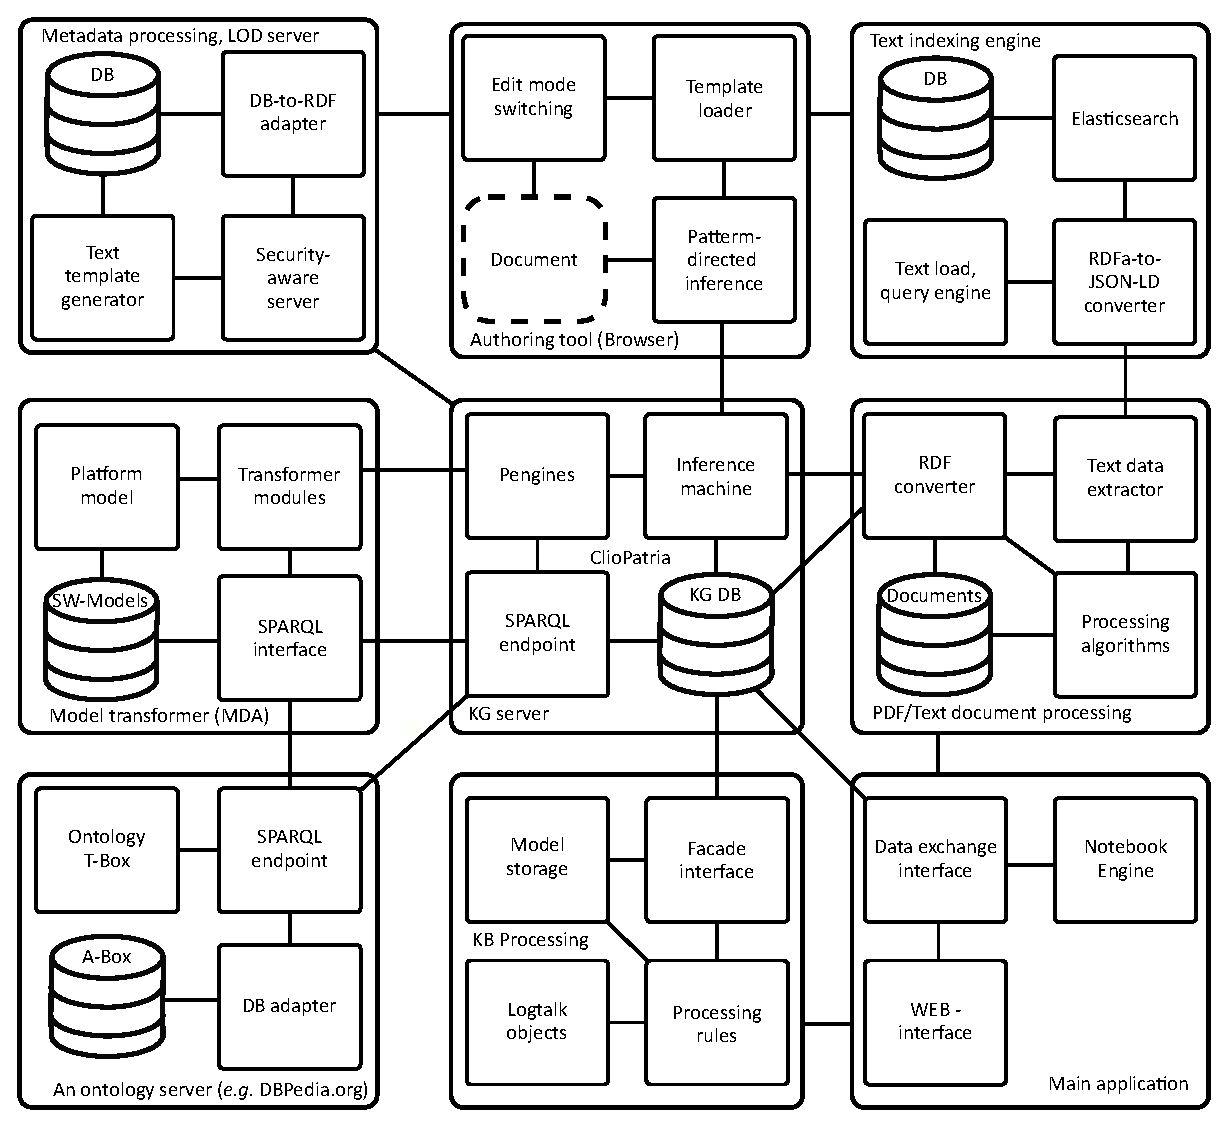
\includegraphics[width=0.9\linewidth]{architecture-mda-lod-ext-general.pdf}
  \end{center}
  \begin{center}
      \textbf{Abbreviations}%\\[1ex]
    \end{center}
    \begin{quote}\scriptsize
      % T-Module is Transformation module,
      MDA is Model-Driven Architecture,
      CIM is Computationally Independent Model,
      PIM is Platform Independent Model,
      PSM is Platform Specific Model,
      T-Box is Terminological Box,
      KB is Knowledge Base,
      % A-Box is Instance Box,
      % NGS is Next-Generation Sequencing,
      DB is Database.
    \end{quote}
  \caption{Architecture of application instrumental environment as a set of components}
  \label{fig:arch-services}
\end{figure}
The kernel module of applications is \texttt{KG server} (B2) built on the base of ClioPatria \cite{cliopatria} with web-server and Pengines plug-ins.  ClioPatria is a web-application implemented in SWI-Prolog \cite{swi} being ISO-compliant Prolog implementation.  KG functions are implemented with SW package, supplied in standard SWI-Prolog distribution.  Pengines service enables SW web-applications to utilize logical inference on the server-side \cite{pengines} with browser JavaScript environment integration.  Pengine's knowledge base is extended with the programmer's Prolog modules.  Kernel module stores a common global part of A-~and T-boxes of applications, \emph{i.e.} it is application database.  Other modules provide an application (C3) with services.

Authoring tool (B1) is used to provide document generation, and integration \cite{zont19}.  This tool enables document content and structure inference in the browser utilizing templates and data from other web pages and websites providing LOD\footnote{Abbreviation of Linked Open Data} \cite{lod} capabilities.  Programmer implements a view of an object as a web page with an extended version of RDFa.  The page is generated within any programming runtime, \emph{e.g.} PHP.  The authoring tool engine collects web page chunks and composes the document as an XHTML page.  This composed page can be stored in a KG as a set of triples and indexed in the Text indexing module (C1), printed with the browser's printing engine, or converted to PDF.  The tool allows the user to change document content in WYSIWYG mode.  Its general structure is defined by changing the template on the server-side.

Text indexing engine (C1) provides a service for storing documents represented as KG triples, JSONs, and BLOBS of any format with corresponding text layers.  This module has two implementations.  One is built on the Sphinx Search engine, and the second is Elasticsearch.  Elasticsearch supports JSON as the only document format and is easily integrated with KG using JSON-LD for triple representation.  Sphinx Search is much faster in text and database records indexing and consumes less RAM as it is implemented in C++.  The choice of an engine depends on the primary document representation used in an application.

BLOB stored documents having no markup (PDFs, scanned documents) usually contain valuable data to be revealed for application use.  The documents could be report data or scientific paper content, DJVU files, or raster images.  Data recognition is implemented in the PDF/Text document processing module (C2), where data processing workers query the Text indexing module for BLOB documents and add recognized text and high-order structure layers.  All obtained layers are stored in the database of C1, and data of general interest are to be converted in triples of KG.

A generalized KG processing is being executed in the KB processing module (B3).  This component denotes a set of rules used to implement the validating and emergent semantics and analysis and synthesis of the new data, including resultant output.  Module A2 is the source of model data (design of domains, UML, problem statement, \emph{etc.}), which is converted and form the T-box of KG.  The conversion is a kind of Model-driven architecture (MDA) implementation.  Transformation is carried out under the control of the Platform model, describing a context of the conversion.  For example, in the case of software source code synthesis, the software platform model is used to implement model objects.

The metadata processing module (A1) denotes the environment capabilities for expressing the semantics out of the data processing modules' output and the input data semantics.  It allows us to store resultant data in KG for further usage in module (B3) for problem-solving and decision-making.  Module A3 denote external services and KG with valuable resources, \emph{e.g.}, DBPedia global objects.

\section{Implementation examples}

In this section, three examples of application implementation are being presented.  The first example is an MDA application in synthesizing a Next-generation sequencing (NGS) investigation environment.  After the invention of methods of NGS and their introduction in the practice of biological systems research, a new direction of molecular genetics is formed, which is referred to as \emph{metagenomics}.  The method allows biologists to describe many new groups of organisms at all taxonomic levels.

\subsection{Next-generation sequencing}
\label{sec:ngs-impl}

The aim of this R\&D \cite{zont19, aicts2020} is to develop software support of the processes of NGS analysis with techniques and software for a visual representation of the computational process for so-called amplicon analysis so that domain specialists would be able to compose computational pipelines, which are executed on distributed heterogeneous computing resources (clouds).  Later, the visual models are used to organize the computational process, data store, and particular NGS data retrieval services.

The tools are based on dataflow representation of various stages of NGS standard operation procedures (SOPs)  formed out of individual operations of Mothur library in Rapidminer studio Java application.  To reflect Mothur's operations, we implemented source code analysis and transformation software.  The C++ sources were analyzed by a Python syntax analyzer based on regular expressions and a top-level algorithm, generating a \verb|TTL| source of KG representing Mothur modules' interfaces.  That was a Computation-independent model (CIM) in the implemented MDA.  CIM transformed into the Platform-independent model (PIM), represented Mothur's modules as dataflow modules, mainly differencing parameters to input/output dataflow ports and parameters.  The Platform-specific model (PSM), \emph{i.e.}, models of Java sources of the dataflow blocks, was constructed, in turn, from PSM.

All transformations were carried out with an object-oriented (OO) Logtalk programming environment representing modules that logically infer new data descriptions of the target objects.  Thanks to OO, the transformation has two levels of abstraction in its representation.  The higher one is a network of objects sending messages via their interfaces.  At the lower one, rules analyze and produce new conclusions on generated object properties.

The PSM objects must have an order in their description as they represent a model of source code to be generated.  The order is organized with blocks of \verb|assert|ed statement and subobjects sequences referencing KG elements.  Blocks can be appended and pretended with new elements.  At the rendering sources stage, the three blocks are traversed in-depth.  It leverages the known \verb|llvmlite| source code generation approach.  Figure~\ref{fig:block-seq} shows the main idea behind PSM object synthesis.
\begin{figure}
  \centering
\begin{multicols}{2}
\begin{minted}[fontsize=\scriptsize]{logtalk}
:- object(class, specializes(code_block),
   imports([named])). % Category of named entities
:- public([classlist/1, methods/1, attributes/1]).
% . . . . . . . . . . . . . .
renderitem(Item, Result):-      % proceed with default
    ^^renderitem(Item, Result). % rendering
render(Result):-         % Source generator
    ^^render(Name),      % implemented in a category
    ( ::item(classlist(List)) ->
     % . . . . . . . . . . .
        [Name]) ),
    ( ::item(attributes(Attributes))->
     % . . . . . . . . . . .
        [DefAttrList]),
      Attributes::items(InstanceAttrs),
      findall(S, ( % initialize attributes
         % . . . . . . . . .
         ), AttrAssigns),
        root::unindent,
        AttrList=[ConstructorDef|AttrAssigns];
         % . . . . . . . . .
        AttrList=[ConstructorDef, Pass] ),
    ( ::item(methods(Methods))-> % If any ...
      Methods::render(MethodList);
      MethodList=[] ),
    lists::append(AttrList,MethodList,StringList),
    root::unindent, Result=[Signature|StringList].
:- end_object.
\end{minted}
      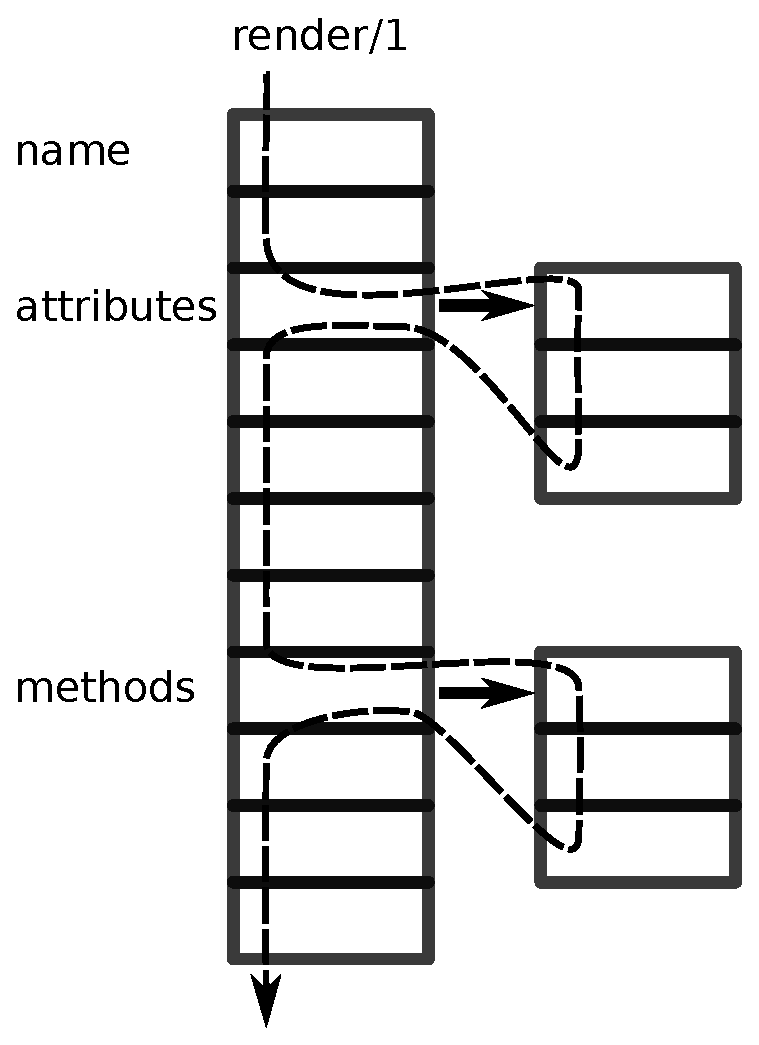
\includegraphics[width=0.7\linewidth]{code_block_class.pdf}
\end{multicols}
  \caption{Procedure of dataflow module source code model synthesis}
  \label{fig:block-seq}
\end{figure}
This example of the application of KG utilizes strongly the property of data representation flexibility for description of the software object model data as well as one central point of data store and access.  The disadvantageous properties of RDF, namely, the weak expressiveness with triples, was neglected by predicate and object encapsulation.

\subsection{Education document authoring}
\label{sec:doc-impl}

This project \cite{authoring} is aimed at the construction of an environment for document authoring out of user-editable template elements, database query results, LOD-compliant web pages, and other document data.  The target document is a web page where content is inferred while loaded by the browser.

All document elements are either context structures or templates filled with other elements.  A context is an RDF hierarchical representation of a document data structure, providing data to be filled in a current rendered template.  The document is rendered from its main template.  All elements are SW resources.  Templates can contain JavaScript subroutines for implementing special services, for example, table of contents out of CSS \verb|class| labeled subsections of the generated document.

All elements are stored in a KG as triples and as LOD-compliant web pages, and according to SW considerations, all of them form a distributed KG.  Data access differentiation by security model is implemented programmatically as the web pages disallow access to the restricted information.  SW has special predicates for describing a possibility and location of a private data sub-KG in the open part.

In Figure~\ref{fig:auth-code}, we presented our small syntactic extension of RDFa for referring template parts.  A namespace \textbf{taa} was added to define a markup interpreted as XHTML tree manipulation in the image and likeliness of open-source ZPT\footnote{Abbreviation of Zope Page Template}.  Arguments of \verb|taa:content| are subcontexts (\verb|title| and \verb|neg-UMK|) of a current template under rendering.
\begin{figure}
  \centering
\begin{minted}[escapeinside=||,fontsize=\small]{text}
<html lang="ru" xmlns=http://www.w3.org/1999/xhtml
|\GB{xmlns:taa}|=http://irnok.net/engine/rdfa-manipulation
xml:lang="ru" metal:define-macro="page">
<head> . . . . </head>
<body prefix="rdf: http://www.w3.org/1999/...-ns# foaf: http://xmlns.com/foaf/...
imei: imei.html# course: https://irnok.net/college/plan/01..16-...\
% D0\%BA_PB-SM.plm.xml.xlsx-....2.3.1.html#"  resource="#post"
typeof="schema:CreativeWork sioc:Post prov:Entity">
<!-- The application control panel -->

<main lang="ru" resource="#annotation" typeof="oa:Annotation" id="main-doc-cnt">
<div property="oa:hasTarget" resource="#course-work-prog"></div>
<article property="oa:hasBody" typeof="foaf:Document curr:WorkingProgram"
         resource="#course-work-program" id="main-document">
  <div |\GB{taa:content}|="imei:title-page"></div>
  <div |\GB{taa:content}|="imei:neg-UMK"></div>
  <section id="TOC" class="break-after"> <h2>Table of Contents</h2>
    <div id="tableOfContents"></div>
  </section>
  <section id="course-description" resource="#description"
           property="schema:hasPart" typeof="schema:CreativeWork">
    <div property="schema:hasPart" resource="#purpose"
         typeof="dc:Text cnt:ContentAsText" >
      <div property="cnt:chars" datatype="xsd:string">
        <h2 property="dc:title" datatype="xsd:string">
           Aims and objectives of the discipline (module)</h2>
        <p>The aim of teaching the discipline ...</p>
      </div>
   </div>
  . . . . . . . .
\end{minted}
  \caption{Part of a template representation}
  \label{fig:auth-code}
\end{figure}

For document markup (document data representation), the following vocabularies are used:
\begin{itemize}
  \item Friend-of-a-friend (\textbf{foaf}), agent information: individuals, legal entities, program agents;
  \item Provenance (\textbf{prov}), references between documents;
  \item Dublin Core (\textbf{dc}), web page annotation mark up;
  \item DBPedia resource (\textbf{dbr}), references to instant objects and classes;
  \item Schema.org (\textbf{schema}), Google, Yandex, Yahoo, \emph{etc}. searchable objects, structural elements;
  \item The Bibliographic Ontology (\textbf{bibo}), literature reference mark up.
\end{itemize}

The general logical structure (sections, subsections, \emph{etc.}) are represented with Open Annotation (\textbf{oa}) vocabulary originally used for annotation of already existing content. The generated document conversion into PDF and other formats is carried out under the control of \textbf{oa}.  HTML5 default tag structures are used for visual sectioning and style definition.

The \textbf{oa} vocabulary is also used to define parts of a document, which allow interactive editing after the document has been rendered.  The obtained changes are fixed in a commit as new resources, and the containing document obtains new IRI fixing all the set of resource changes.

\subsection{Web GIS on the base of a knowledge graph}
\label{sec:gis-impl}

Project \cite{gisviewer} devoted to investigating capabilities of SW and KG technologies in representation spatially distributed data (GIS\footnote{Abbreviation of Geographical Information System}-data).  The fault data \cite{lunina,afs} are chosen as a subject for representation and publishing in this investigation.  In geology, researchers accumulate data obtained after event observations, \emph{e.g.}, earthquakes, landslides, by analyzing remote sensing data and results of field works.  The obtained data are processed and interpreted, setting new attributes to a fault or refinement of their values.  According to the geological research techniques, additional information is associated with attributes, clarifying their values.  Such clarification comprises precision characteristics, measurement conditions, reliability assessment, paper references, and published fault data.

GIS represents spatial data in semantic-defined layers.  For each object of a GIS layer, one can associate a set of attribute values of auxiliary data.  The attribute set is the same for each object of a layer, regardless the attribute's value is defined or not.  Empty values are represented as ``\texttt{null}''s.  In the case of geological exploration, when many attributes are undefined, this approach leads to sparsely filled tables.  In this case, structure modification and data analysis algorithms are required to utilize additional data checking stages when using standard relation operations (SELECT, UPDATE, DELETE).

Web publication applications, like information systems, implement filtering functions, differentiating the value attributes and their metadata.  Screen widgets label names either defined in application configuration or figured out from the attribute names.  Lack of vocabulary formal domain definition forces developers to spend more effort on user interface implementation.

In this project, we constructed a Web-application using contemporary Web and SW technologies for rendering a fault map, in which visual content is controlled by data filters implemented as SPARQL queries to KG representing fault data.  For this purpose, data conversion from the tabular form to KG was carried out, a CliopPatria server for data storage was installed, and data viewers for the triple sets for a typical subject (a fault) have been implemented.  In Figure~\ref{fig:gis-ex} an example of the filtering and a selected object data viewing form is presented.
\begin{figure}
  \centering
  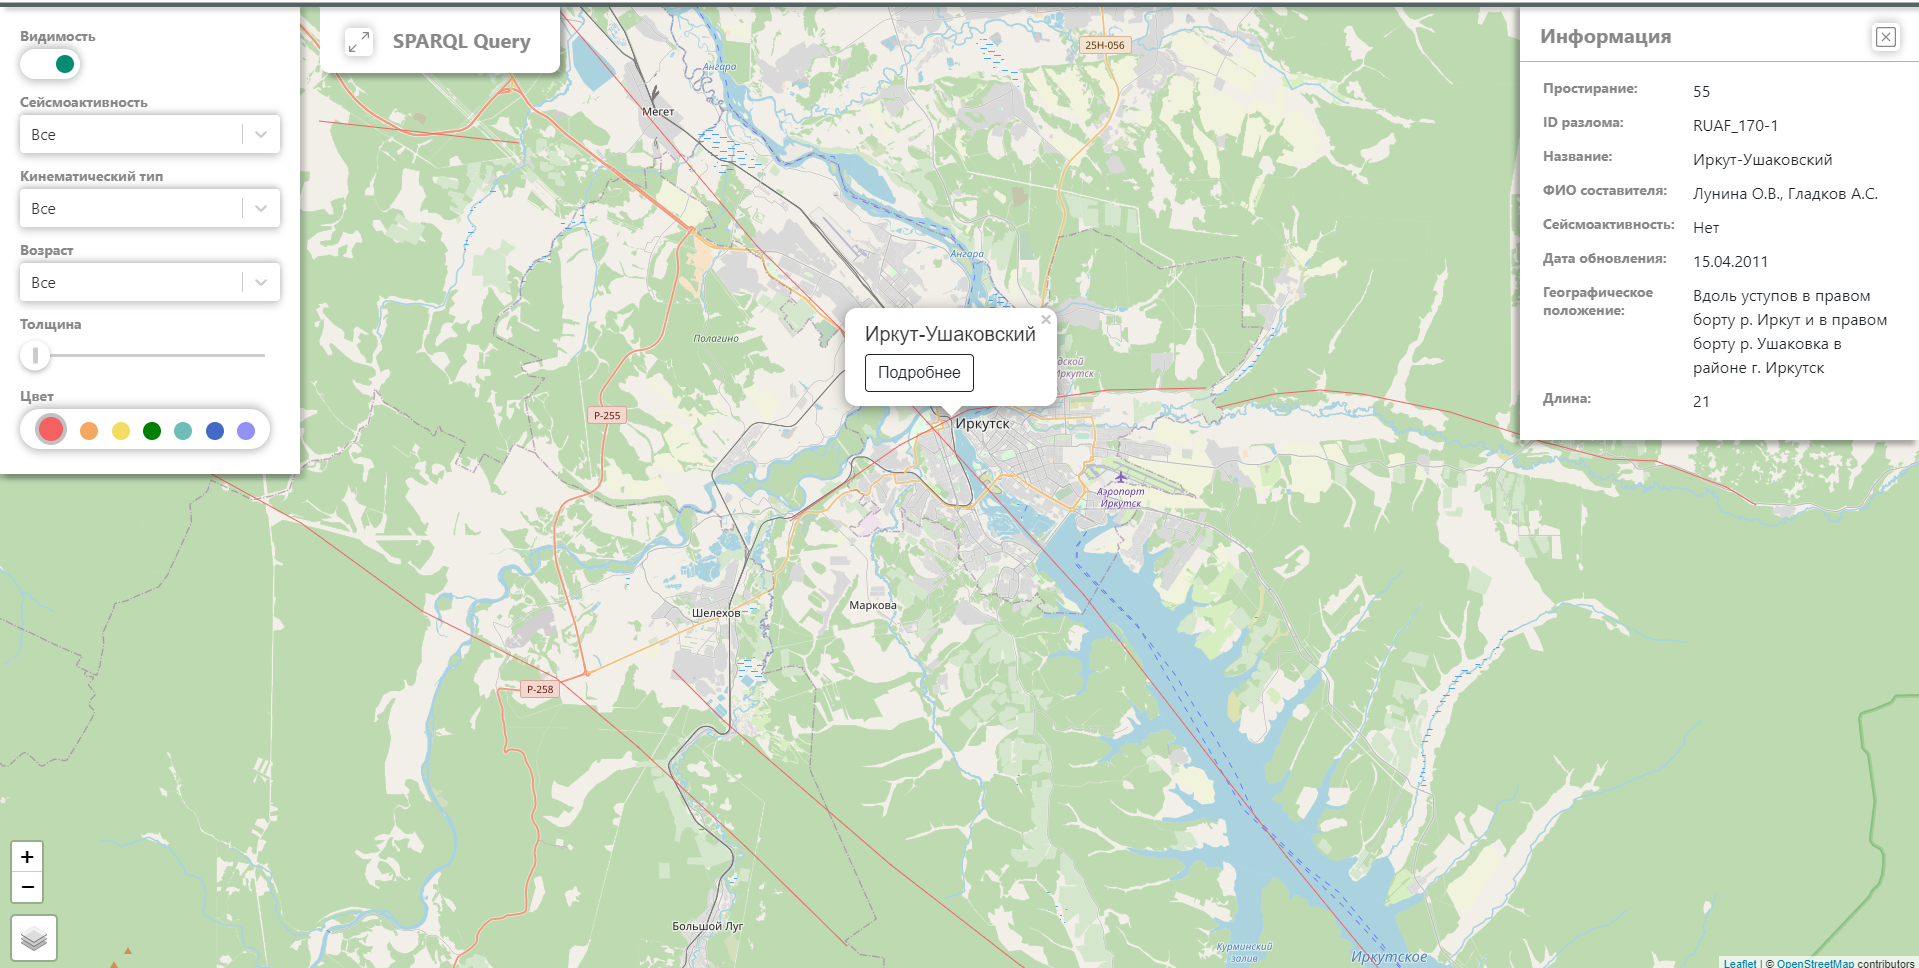
\includegraphics[width=\linewidth]{faults-leaflet-doc.png}
  % \caption{Viewer window showing description of a fault}
  \caption{Example of GIS rendering of KG data}
  \label{fig:gis-ex}
\end{figure}

The proposed technology and software allow one to construct Web-GIS systems for research communities, as they support constant data accumulation, aggregation, and analysis thanks to the properties of knowledge graph (KG) data storage and processing.

\section*{Conclusion}
\label{sec:disc}

Standardized forms of basic concepts of data representation and processing in Semantic Web (SW) research were considered in this paper.  Special attention has been paid to reviewing Knowledge Graph (KG) data storage and processing in the scientific data processing software.

We did not consider analogous R\&D as it was already reviewed in the corresponding publications.  Another point of our R\&D is improving existing technologies, data, and software with our tools, such as MDA.  We present a review of obtained SW and KG technologies application experience.  The main one is the powerful application integration capabilities, where all the set of implemented software forms a distributed environment of data processing.  The main requirement is that the data representation at storage services and in the protocol implementations should obey SW and KG standards.

The main advantages of these technologies for the software developer are semantic markup and generic properties of KG, especially a possibility to postpone formal data structure definition as such declarative set-based data can be processed with a rule-based inference engine.  Scientific community results in domain description in standardized vocabularies (ontologies), user communities aggregating and formalizing data on real-world objects form a productive background for problem space description and,  in its turn, a common basis for application integration, which results in a cumulative effect of aggregation of developed software in a complex distributed data processing system and environments.

Further development of the technologies includes the following directions of great interest:
\begin{itemize}
\item Fibered representation of KG to support consistency and completeness check by reflecting A-Box entities and their relations to template domain models;
\item Investigate expressive capabilities of Logtalk programming language as an instrument of knowledge (rules) representation for KG processing modules;
\item Adding extended document analysis services \cite{shigpaper} to the environment (section~\ref{sec:architecture}), which are developed in our research group;
\item Improve integration techniques with metamodel presentation of the execution environment.
\end{itemize}

\begin{acknowledgments}

The results were obtained within the state assignment of the Ministry of Education and Science of Russia, the project ``Methods and technologies of a cloud-based service-oriented digital platform for collecting, storing and processing large volumes of multi-format interdisciplinary data and knowledge based on the use of artificial intelligence, a model-driven approach, and machine learning'', No.~FWEW-2021-0005 (State registration No.~121030500071-2).

The results were obtained with the use of the network infrastructure of the Telecommunication center of collective use ``Integrated information-computational network of Irkutsk scientific-educational complex'' (\url{http://net.icc.ru}).

The~R\&D on GIS-viewer of faults involved the Centre of Geodynamics and Geochronology equipment at the Institute of the Earth's Crust, Siberian Branch of the Russian Academy of Sciences (grant No.~075-15-2021-682).   This study direction was partially carried out within the basic budgetary research project ``Modern geodynamics, mechanisms of destruction of the lithosphere and hazardous geological processes in Central Asia'', No.~FWEF-2021-0009.

The~development of the~infrastructure for Mothur command transformation to Rapidminer dataflow diagram is supported by the Irkutsk scientific center of Siberian Branch of Russian Academy of Sciences, grant No 4.2.

\end{acknowledgments}
%%
%% Define the bibliography file to be used
% \bibliography{sample-ceur}

\begin{thebibliography}{99}


\bibitem{tbl} Tim Berners-Lee, James Hendler, and Ora Lassila.  The semantic web: A new form of web content that is meaningful to computers will unleash a revolution of new possibilities.  Scientific American, Vol.~05, 2001.

\bibitem{hogan} A.~Hogan, E.~Blomqvist, M.~Cochez, C.~D’Amato \emph{et al}. Knowledge Graphs, 2020. \url{https://arxiv.org/abs/2003.02320v5}

\bibitem{lod} C.~Bizer, T.~Heath, T.~Berners-Lee, Linked Data -- The Story So Far.  Int. J. Semantic Web Inf. Syst., 5 (2009), pp.~1--22. \doi{10.4018/jswis.2009081901}

\bibitem{lunina} O.~V.~Lunina.  The digital map of the Pliocene–Quaternary crustal faults in the Southern East Siberia and the adjacent Northern Mongolia.  Geodynamics \& Tectonophysics.  V.~7(3) (2016).  pp.~407-434. (in Russian) \doi{10.5800/GT-2016-7-3-0215}

\bibitem{afs} A.~A.~Gladkov, O.~V.~Lunina. Cartographic service ``Activetectonics''. \url{http://activetectonics.ru/} (access date: 20-Sep-2021)

%\bibitem{foss} M.~Leidig, R.~Teeuw. Free software: A review, in the context of disaster management.  International Journal of Applied Earth Observation and Geoinformation, 42 (2015), pp.~49-56. \doi{10.1016/j.jag.2015.05.012}.

%\bibitem{lgd} C.~Stadler, J.~Lehmann, K.~Höffner, S.~Auer. LinkedGeoData: A core for a web of spatial open data. Semantic Web 3 (2012) 333–354. \doi{10.3233/SW-2011-0052}

%\bibitem{geolink} M.~Cheatham, A.~Krisnadhi, R.~Amini, P.~Hitzler, \emph{et al}. The GeoLink knowledge graph, Big Earth Data, 2:2 (2018), pp.~131-143. \doi{10.1080/20964471.2018.1469291}

%\bibitem{abid} T.~Abid, H.~Zarzour. Integrating linked open data in a geographical information system.  Procs.  of. International Conference on Information Technology for Organization Development. Oct 19-20, 2014, University of Tebessa, Tebessa, Algeria (2014).

%\bibitem{iwaniak1} A.~Iwaniak, I.~Kaczmarek, M.~Strzelecki, J.~Lukowicz, P.~Jankowski. Enriching and improving the quality of linked data with GIS. Open Geosciences, Vol.~8, 1~(2016) pp.~323-336. \doi{10.1515/geo-2016-0020}

%\bibitem{iwaniak17} A.~Iwaniak, M.~Leszczuk, M.~Strzelecki, F.~Harvey, I.~Kaczmarek. A Novel Approach for Publishing Linked Open Geodata from National Registries with the Use of Semantically Annotated Context Dependent Web Pages.  International Journal of Geo-Information. 6, 252 (2017). \doi{10.3390/ijgi6080252}

\bibitem{zont19} E.~Cherkashin, A.~Shigarov, V.~Paramonov. Representation of MDA transformation with logical objects.  International Multi-Conference on Engineering, Computer and Information Sciences (SIBIRCON), Novosibirsk, Russia. (2019) 0913--0918 \doi{10.1109/SIBIRCON48586.2019.8958008}

\bibitem{aicts2020} Evgeniy Cherkashin, Alexey Shigarov. Construction techniques of Baikal microbiome research information-computational environment.  Proceedings for 1st International Workshop on Advanced Information and Computation Technologies and Systems. Irkutsk, Russia, December 7-11, 2020. CEUR-WS.org, online \url{http://ceur-ws.org/Vol-2858/paper2.pdf} (access date: 12-Dec-2021)

\bibitem{authoring} E.~Cherkashin, A.~Shigarov, V.~Paramonov, A.~Mikhailov, Digital archives supporting document content inference, Procs.  of 42-nd International Convention on Information and Communication Technology Electronics and Microelectronics (MIPRO), May 20–24, 2019.  pp. 1037-1042. \doi{10.23919/MIPRO.2019.8757196}

\bibitem{gisviewer} E.~Cherkashin, O.~Lunina, L.~Demyanov, A.~Tsygankov. Web-GIS viewer for active faults data represented as a knowledge graph.  Proceedings for 4th Scientific-practical Workshop Information Technologies: Algorithms, Models, Systems. Irkutsk, Russia, September 14, 2021. CEUR-WS.org, online \url{http://ceur-ws.org/Vol-2984/paper8.pdf} (access date: 12-Dec-2021)

\bibitem{cliopatria} J. Wielemaker, W. Beek, M. Hildebrand, J. Ossenbruggen, ``ClioPatria: A
  SWI-Prolog infrastructure for the Semantic Web,'' Semantic Web.
  Vol. 7(5).  P. 529--541 (2016) \doi{10.3233/SW-150191}

\bibitem{shigpaper} Dorodnykh N.O., Yurin A.Y., Shigarov A.O. (2020) Conceptual Model Engineering for Industrial Safety Inspection Based on Spreadsheet Data Analysis.  In: Simian D., Stoica L. (eds) Modelling and Development of Intelligent Systems.  MDIS 2019.  Communications in Computer and Information Science, vol 1126.  Springer, Cham. \doi{10.1007/978-3-030-39237-6_4}

\bibitem{pengines} {Torbj{\"{o}}rn Lager, Jan Wielemaker. Pengines: Web Logic Programming Made Easy.  Theory and Practice of Logic Programming.  Vol.~14, No.~4-5. pp.~539--552. 2014. \doi{10.1017/S1471068414000192}

\bibitem{swi} Jan Wielemaker, Tom Schrijvers, Markus  Triska, Torbj\"o{}rn} Lager. SWI-Prolog. Theory and Practice of Logic Programming, Vol.~12, No.~1-2, pp.~67--96, ISSN~1471-0684.

\end{thebibliography}
% \section{Online Resources}

% The sources for the viewer are being developed at Github, URL:~\url{https://github.com/De17eon/GRL}.

\end{document}

%%
%% End of file


%%% Local Variables:
%%% mode: latex
%%% TeX-master: "paper-aicts-cherkashin.tex"
%%% End:
